\documentclass[crop, tikz]{standalone}
\usepackage{tikz}

\usetikzlibrary{positioning}

\begin{document}
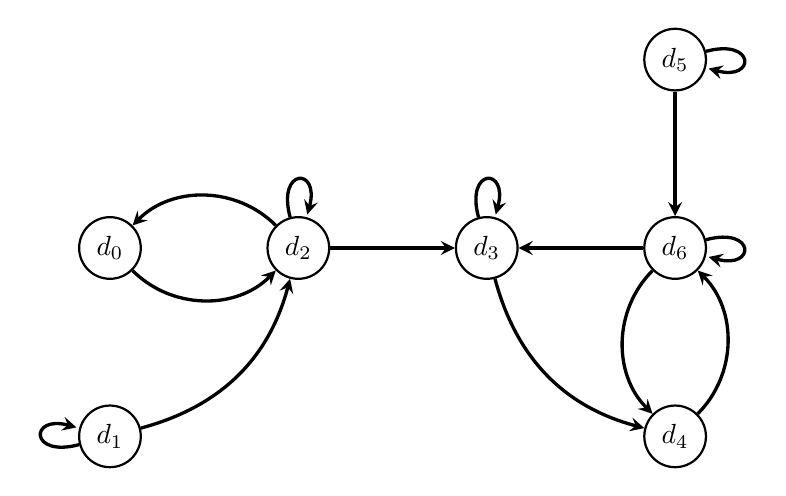
\begin{tikzpicture}
	\node[circle, thick, draw] (0) {$d_0$};
	\node[circle, thick, draw, below = 4.5em of 0] (1) {$d_1$};
	\node[circle, thick, draw, right = 4.5em of 0] (2) {$d_2$};
	\node[circle, thick, draw, right = 4.5em of 2] (3) {$d_3$};
	\node[circle, thick, draw, right = 4.5em of 3] (6) {$d_6$};
	\node[circle, thick, draw, above = 4.5em of 6] (5) {$d_5$};
	\node[circle, thick, draw, below = 4.5em of 6] (4) {$d_4$};
	
	\path[-stealth, very thick] (0) edge [bend right=45] (2);
	\path[-stealth, very thick] (2) edge [bend right=45] (0);
	\path[-stealth, very thick] (1) edge [bend right] (2);
	\path[-stealth, very thick] (1) edge [->, >=stealth, loop left] (1);
	\path[-stealth, very thick] (2) edge [->, >=stealth, loop above] (2);
	\path[-stealth, very thick] (3) edge [->, >=stealth, loop above] (3);
	\draw[-stealth, very thick] (2) -- (3);
	\path[-stealth, very thick] (3) edge [bend right] (4);
	\draw[-stealth, very thick] (5) -- (6);
	\draw[-stealth, very thick] (6) -- (3);
	\path[-stealth, very thick] (6) edge [bend right=45] (4);
	\path[-stealth, very thick] (4) edge [bend right=45] (6);
	\path[-stealth, very thick] (5) edge [->, >=stealth, loop right] (5);
	\path[-stealth, very thick] (6) edge [->, >=stealth, loop right] (6);
\end{tikzpicture}
\end{document}
